\section{Data Flow Diagram}
\vspace{1cm}

\subsection{Level 0 DFD}
The Level 0 DFD delineates boundary interactions of the AyurSpace system. The central
process (0) interfaces to three entities: Mobile User End Device, Firebase Cloud, and
external AI nodes (Plant.id and Google Gemini). Users input credentials, images, and
text queries. The system returns taxonomic confidence arrays and Ayurvedic response text,
whilst syncing profiles securely with the Firebase cloud.

\vspace{1cm}
\renewcommand{\thefigure}{6.1.1}
\begin{figure}[h]
\begin{mdframed}
     \centering
    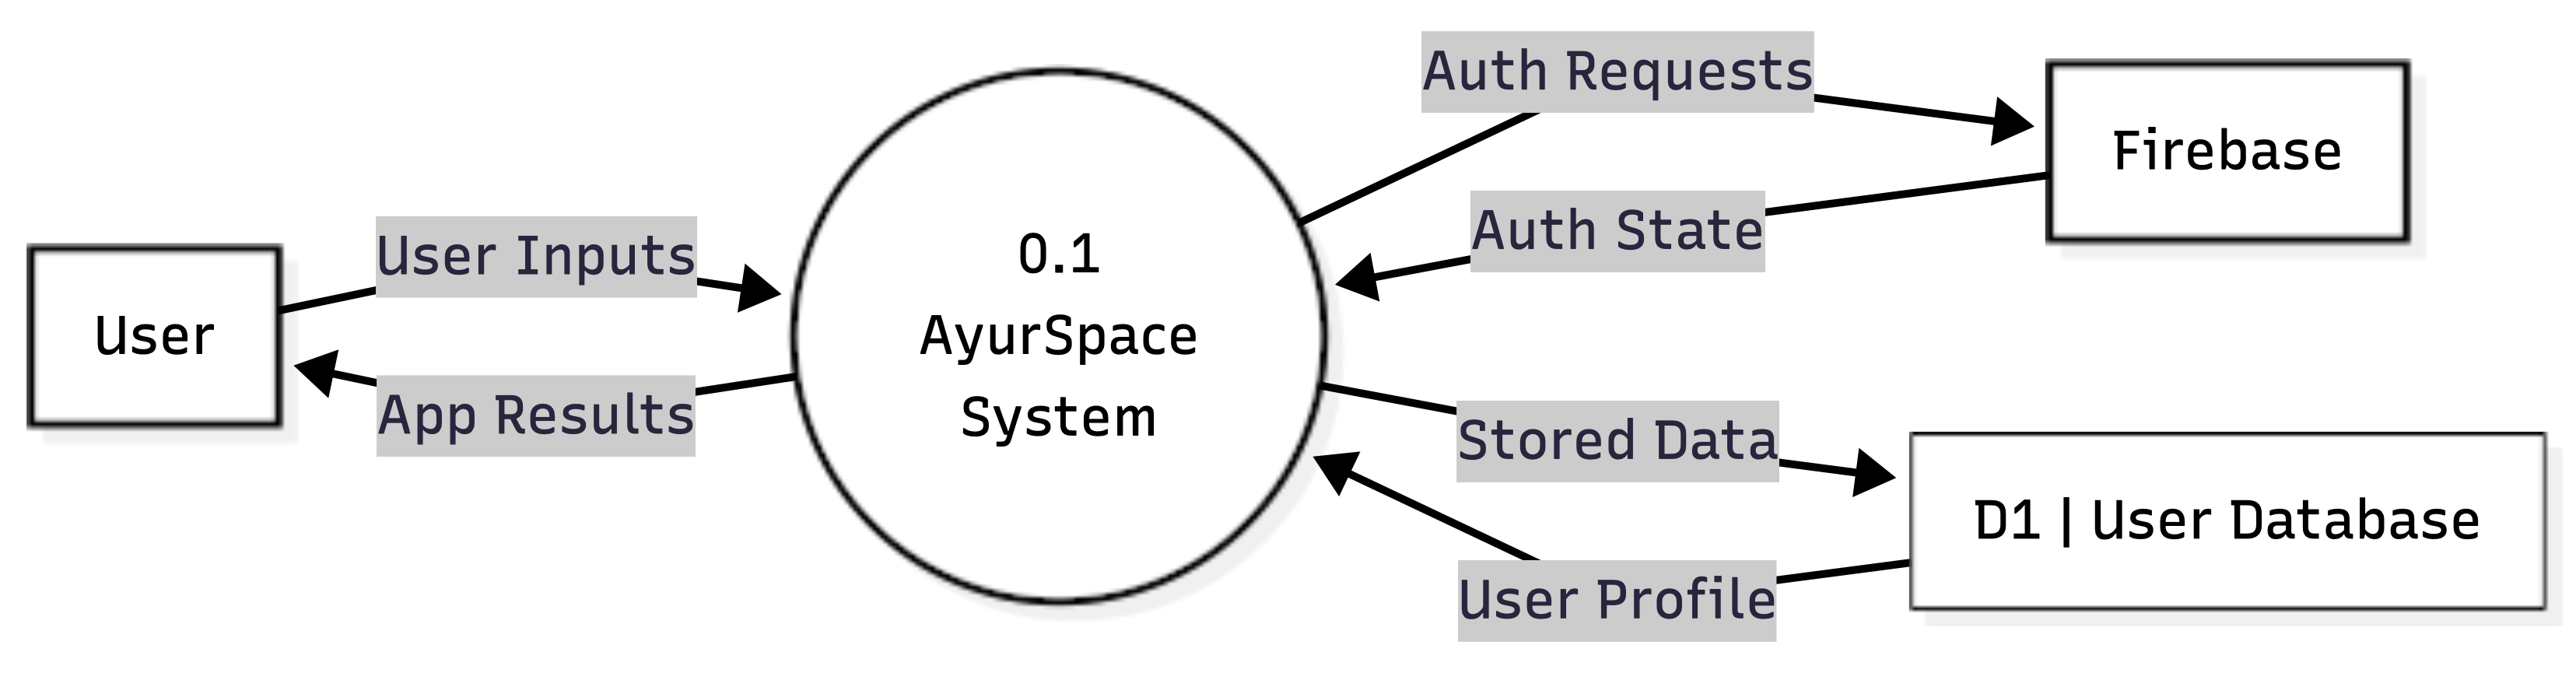
\includegraphics[width=0.7\linewidth,keepaspectratio]{assets/placeholders/placeholder_dfd0.png}
\end{mdframed}
 \caption{Level 0 DFD}
\end{figure}

\newpage
\subsection{Level 1 DFD}
The Level 1 DFD breaks process 0 into dedicated components: Authentication Management
(1.0), Image Processing \& Vision (2.0), Ayurvedic Reasoning Engine (3.0), and Health
Profiling (4.0). Data stores: D1 (User Profiles), D2 (Scan History). Raw images are
translated via external APIs within 2.0, context flows into 3.0 alongside Gemini LLMs,
and profiling calculations merge into reasoning to yield tailored health output.

\vspace{0.5cm}
\renewcommand{\thefigure}{6.1.2}
\begin{figure}[!htbp]
\begin{mdframed}
    \centering
    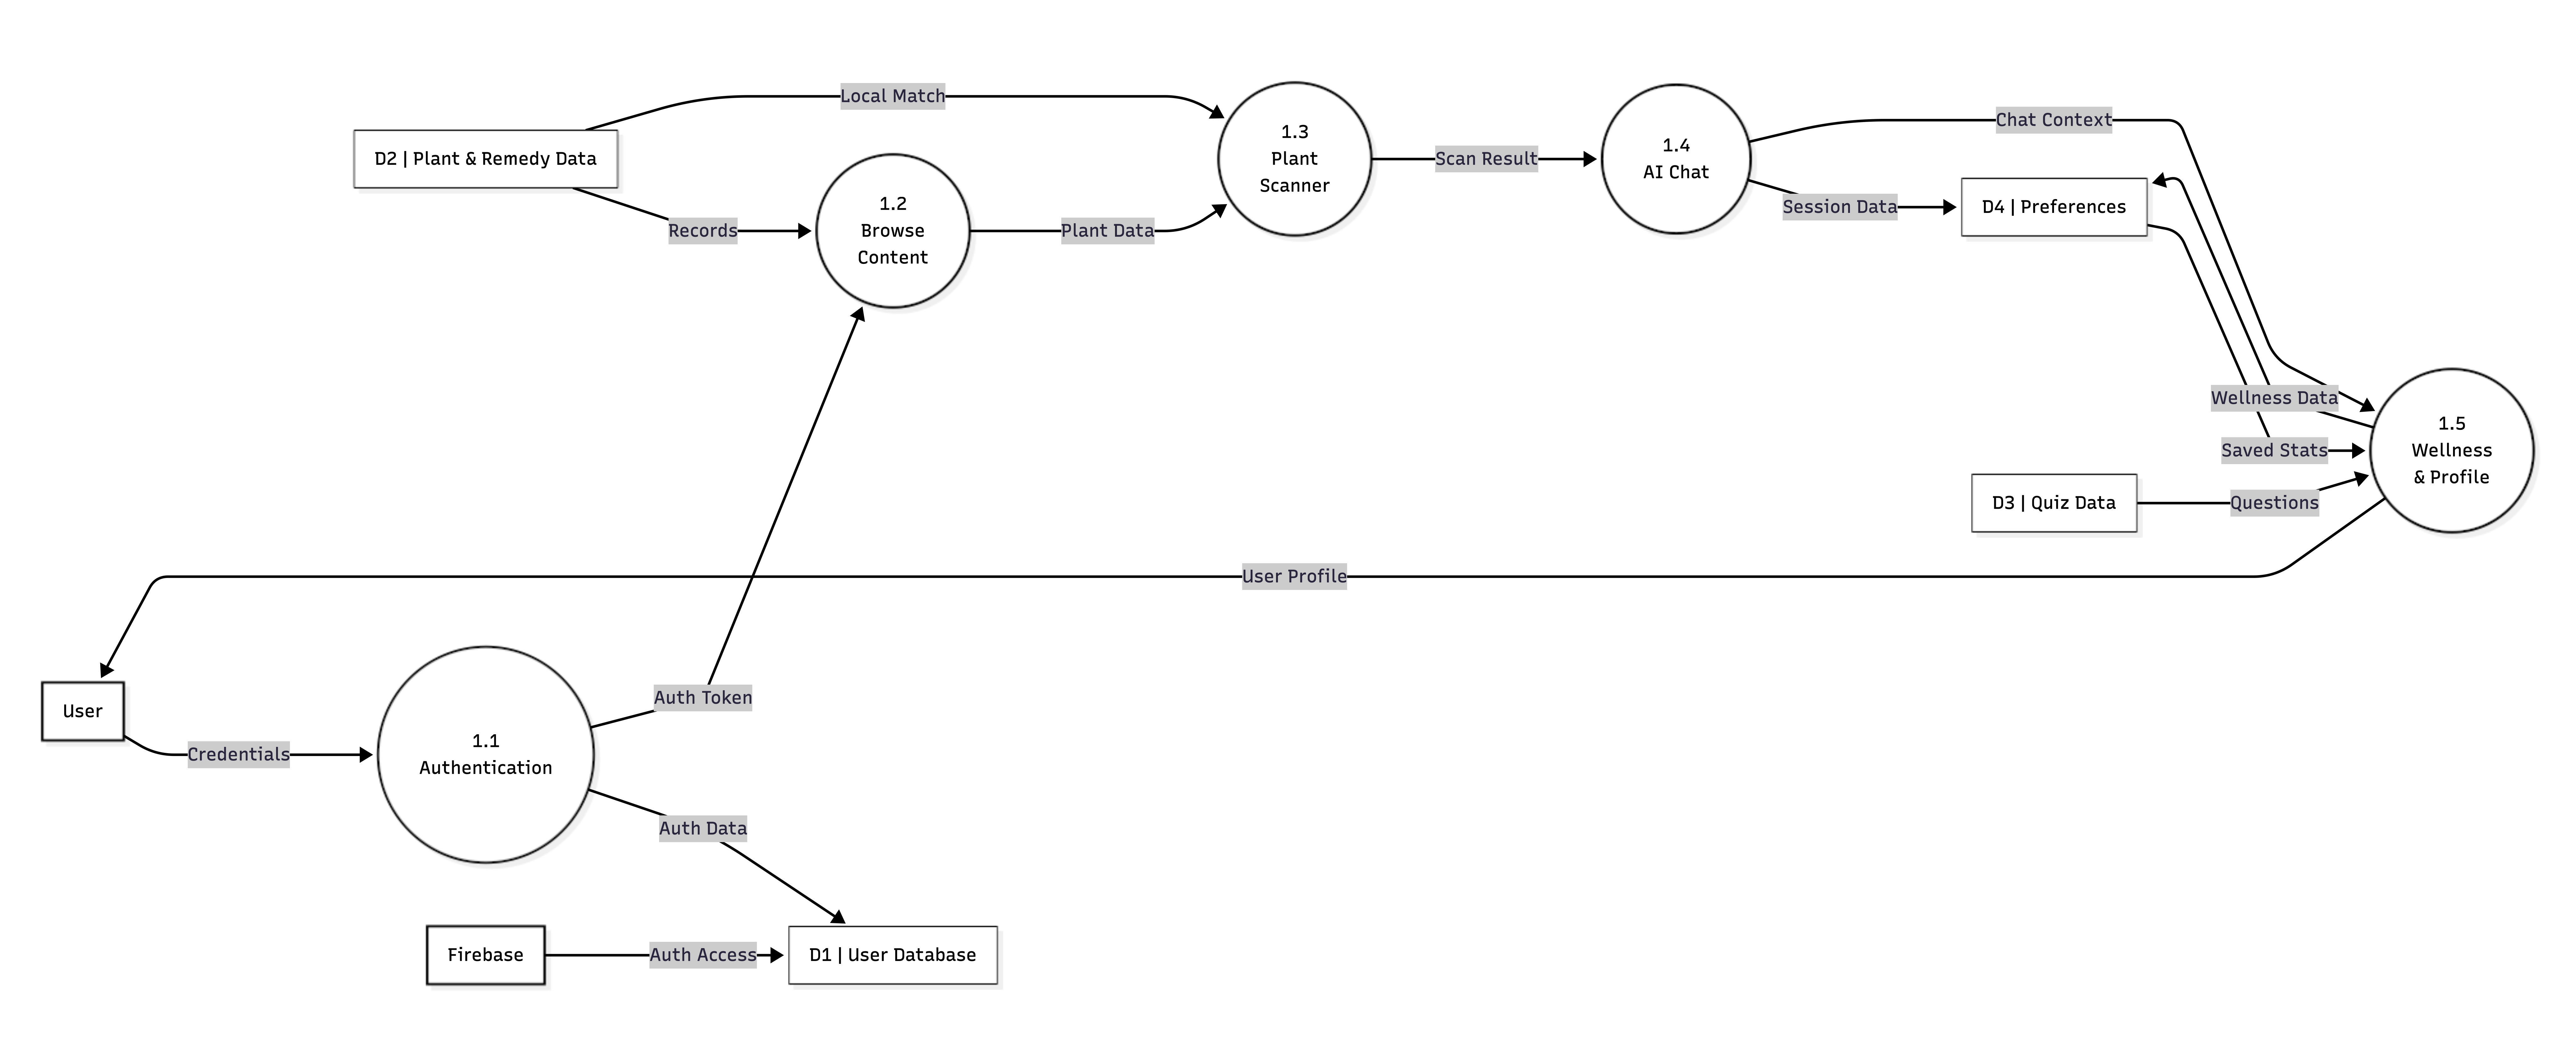
\includegraphics[width=\linewidth,height=0.8\textheight,keepaspectratio]{assets/placeholders/placeholder_dfd1.png}
\end{mdframed}
    \caption{Level 1 DFD}
\end{figure}

\newpage
\section{Flow Chart}
The Flowchart maps in-app navigation behavior. Auth verification $\rightarrow$ Home
Dashboard $\rightarrow$ branches into Scanning (taxonomy confidence gate), Chatting
(Gemini context query with rules), and Assessment (scoring algorithm execution).

\renewcommand{\thefigure}{6.2}
\begin{figure}[!htbp]
\begin{mdframed}
    \centering
   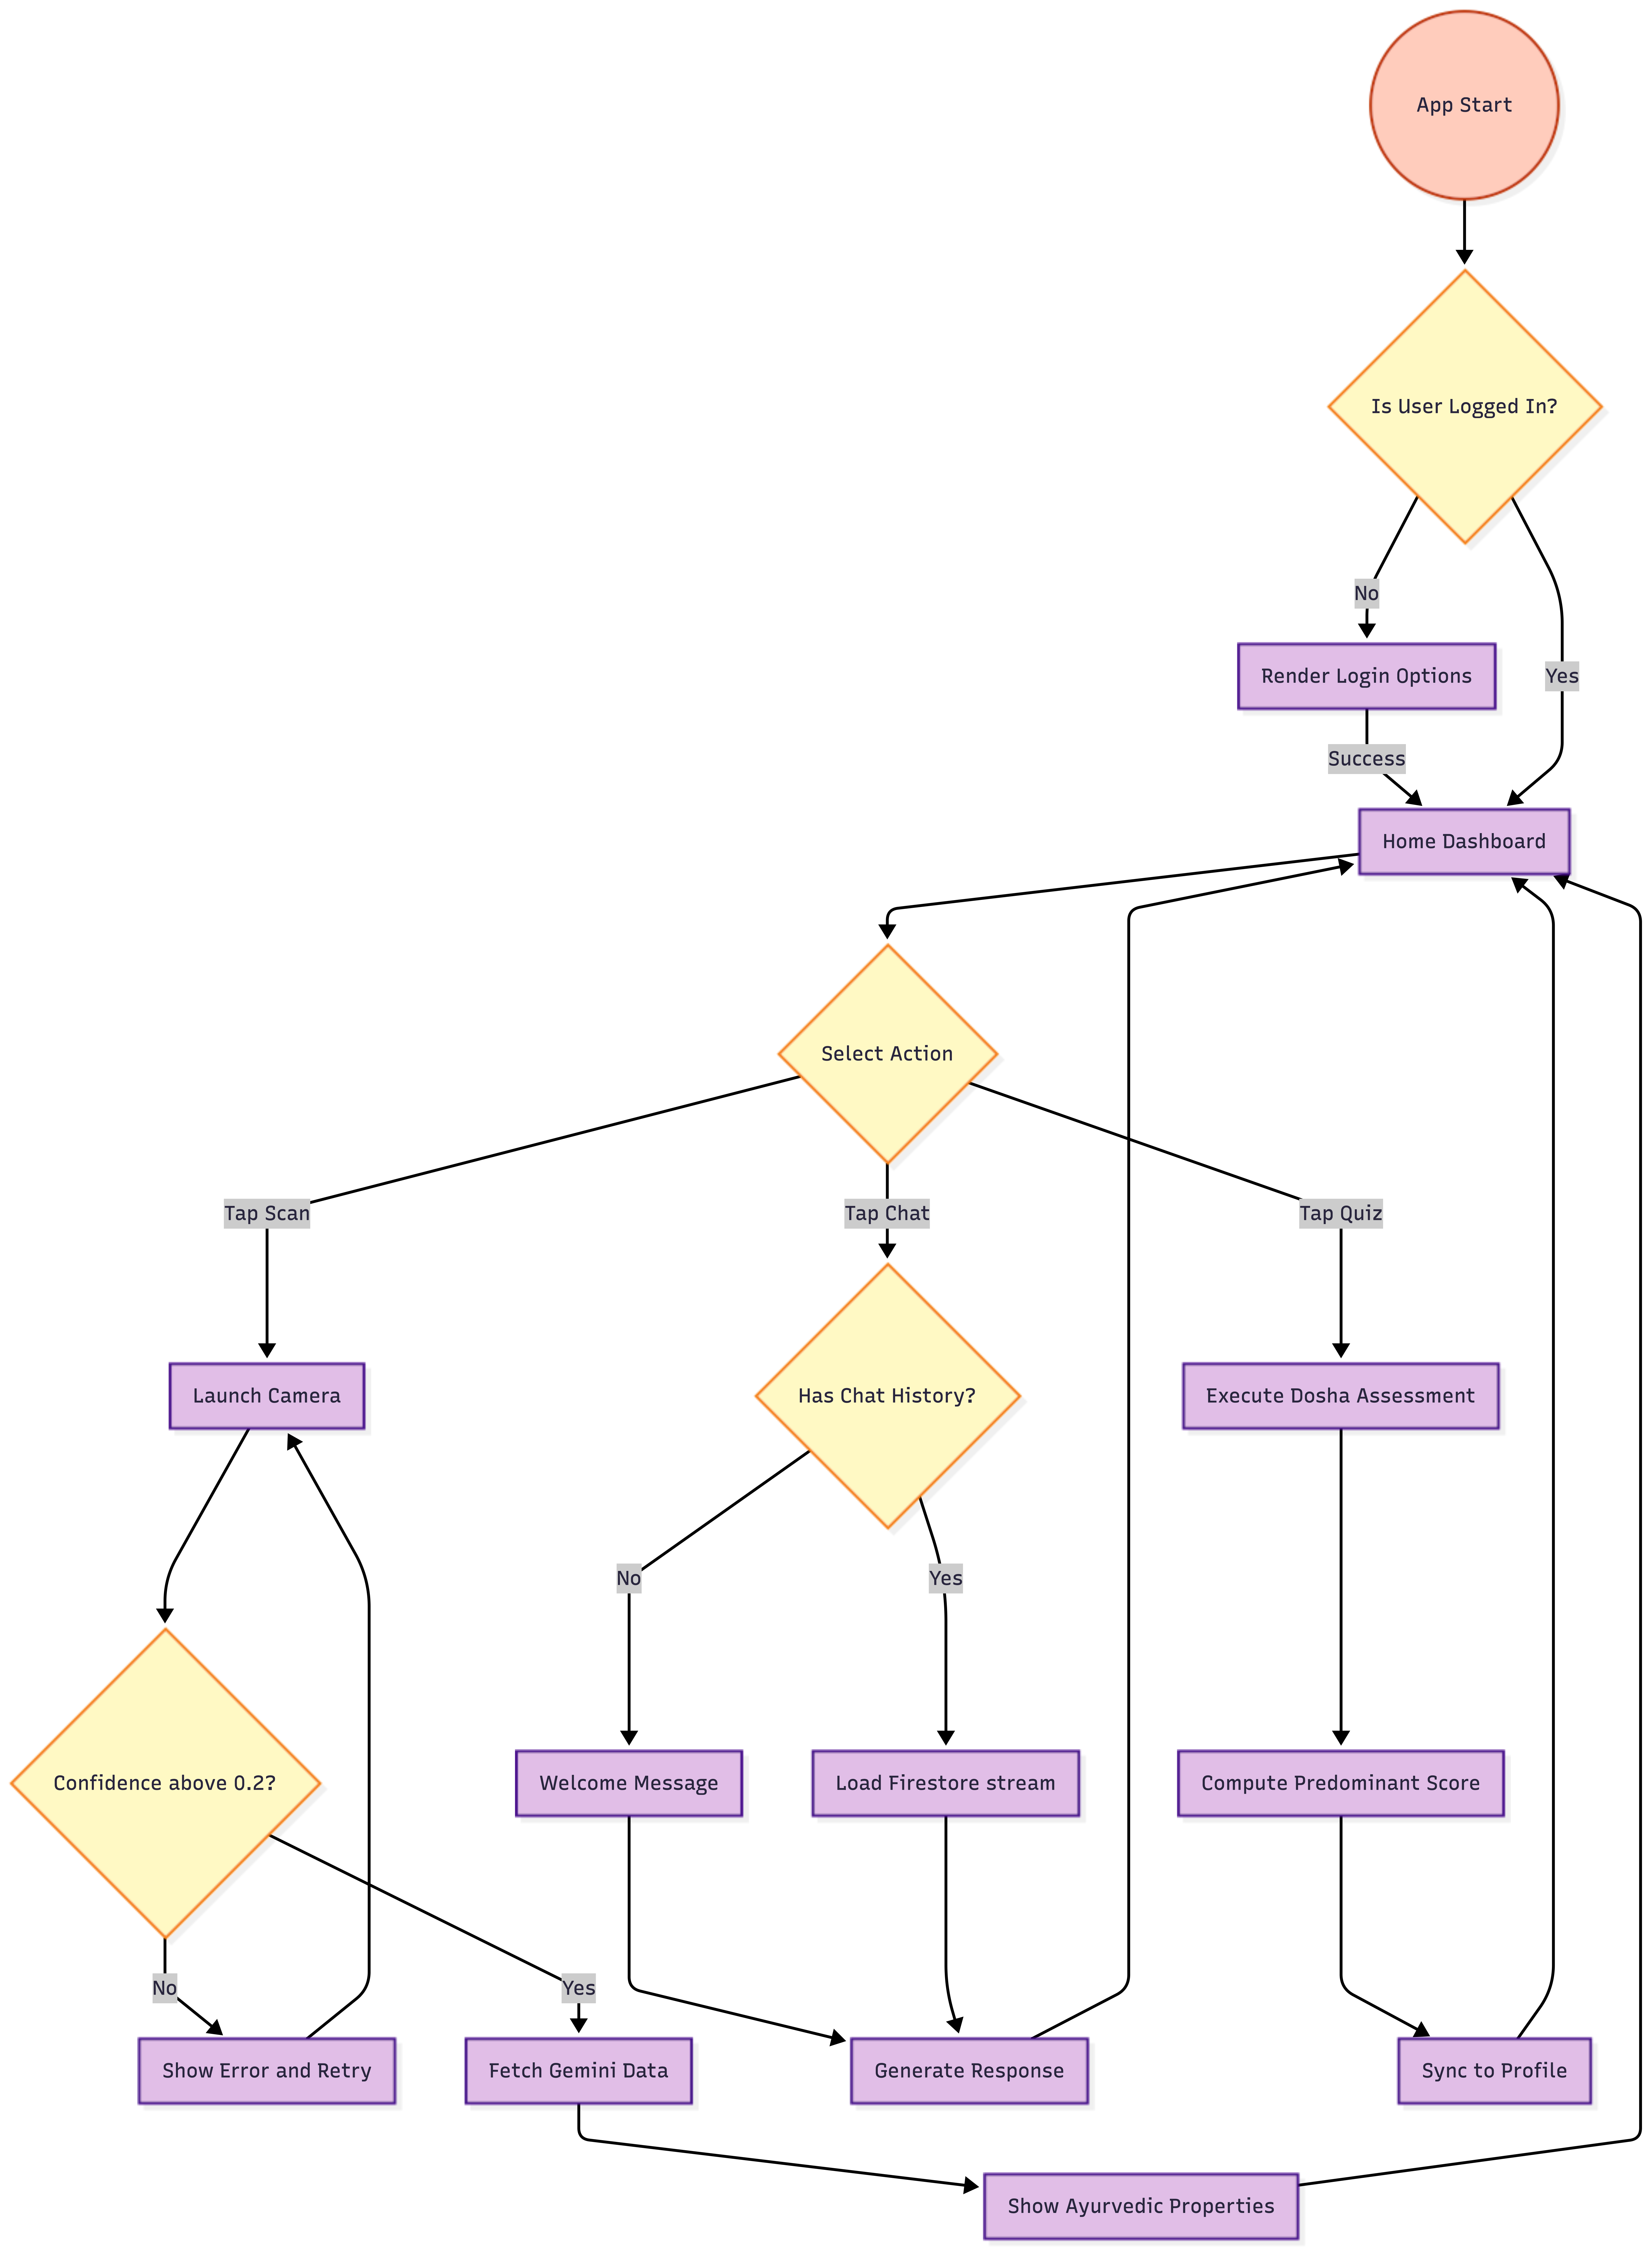
\includegraphics[width=\linewidth,height=0.7\textheight]{assets/placeholders/placeholder_flowchart.png}
\end{mdframed}
\caption{Flow Chart}
\end{figure}
